\uuid{88TT}
\titre{Etude d'une fonction}
\theme{optimisation, fonctions de plusieurs variables}
\auteur{}
\organisation{AMSCC}

\contenu{


\texte{ Soit la fonction $f$ définie sur $\mathcal{D} \subset \R^2$ par 
$$f(x,y) = x^3 + y^3 - 3xy$$
où $\mathcal{D} = \{ (x,y) \in \R^2 \, , \max(|x|,|y|) \leq 2\}$. }

\begin{enumerate}
	\item \question{ Parmi les trois domaines représentés graphiquement ci-dessus, lequel est susceptible de représenter $\mathcal{D}$ ? }
	
	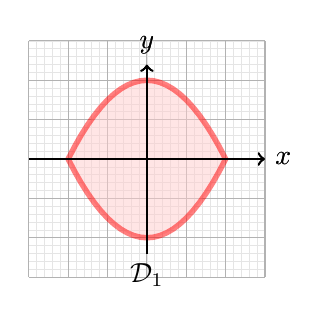
\begin{tikzpicture}[domain=-1:1]
		\draw[->,thick] (-1.5,0) -- (1.5,0) node[right] {$x$};
		\draw[->,thick] (0,-1.2) -- (0,1.2) node[above] {$y$};
		\draw[very thin, style=gray!20,  step=0.1] (-1.5,-1.5) grid(1.5,1.5);
		\draw[thin,gray!60, step = 0.5]  (-1.5,-1.5) grid(1.5,1.5);
		\filldraw[fill=red!20, draw=red, line width = 2pt, opacity = 0.5] plot [domain=-1:1] (\x,{1-\x*\x})  -- plot [domain=1:-1] (\x,{\x*\x-1}) ;
		\draw[->,thick] (-1.5,0) -- (1.5,0) node[right] {$x$};
		\draw[->,thick] (0,-1.2) -- (0,1.2) node[above] {$y$};
		\draw (0,-1.2) node[below]{$\mathcal{D}_1$} ;
	\end{tikzpicture} \hfill
	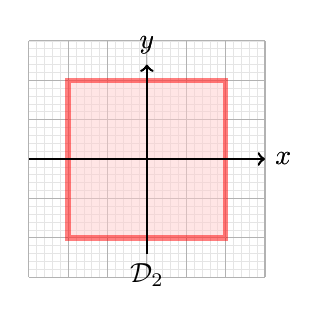
\begin{tikzpicture}[domain=-1:1]
		\draw[->,thick] (-1.5,0) -- (1.5,0) node[right] {$x$};
		\draw[->,thick] (0,-1.2) -- (0,1.2) node[above] {$y$};
		\draw[very thin, style=gray!20,  step=0.1] (-1.5,-1.5) grid(1.5,1.5);
		\draw[thin,gray!60, step = 0.5]  (-1.5,-1.5) grid(1.5,1.5);
		\filldraw[fill=red!20, draw=red, line width = 2pt, opacity = 0.5] (1,1) -- (1,-1) -- (-1,-1) -- (-1,1) -- cycle ;
		\draw[->,thick] (-1.5,0) -- (1.5,0) node[right] {$x$};
		\draw[->,thick] (0,-1.2) -- (0,1.2) node[above] {$y$};
		\draw (0,-1.2) node[below]{$\mathcal{D}_2$} ;
	\end{tikzpicture} \hfill
	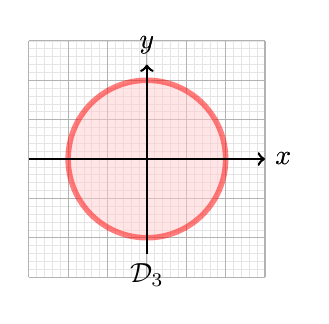
\begin{tikzpicture}[domain=-1:1]
		\draw[->,thick] (-1.5,0) -- (1.5,0) node[right] {$x$};
		\draw[->,thick] (0,-1.2) -- (0,1.2) node[above] {$y$};
		\draw[very thin, style=gray!20,  step=0.1] (-1.5,-1.5) grid(1.5,1.5);
		\draw[thin,gray!60, step = 0.5]  (-1.5,-1.5) grid(1.5,1.5);
		\filldraw[fill=red!20, draw=red, line width = 2pt, opacity = 0.5] (0,0) circle (1) ;
		\draw[->,thick] (-1.5,0) -- (1.5,0) node[right] {$x$};
		\draw[->,thick] (0,-1.2) -- (0,1.2) node[above] {$y$};
		\draw (0,-1.2) node[below]{$\mathcal{D}_3$} ;
	\end{tikzpicture}
	
	\item \question{  L'ensemble $\mathcal{D}$ est-il ouvert dans $\R^2$ ? fermé dans $\R^2$ ? Justifier très brièvement. }
	
	\item\question{  Vérifier que $(0,0)$ et $(1,1)$ sont les deux seuls points critiques de $f$ dans l'intérieur du domaine  $\mathcal{D}$.  }
	\item \question{ La fonction $f$ admet-elle un extremum local sur l'intérieur de $\mathcal{D}$ ? }
	\item \question{ Justifier que $f$ admet un maximum global sur $\mathcal{D}$ et le calculer.  }
\end{enumerate}
}